\documentclass[]{article}
\usepackage{lmodern}
\usepackage{amssymb,amsmath}
\usepackage{ifxetex,ifluatex}
\usepackage{fixltx2e} % provides \textsubscript
\ifnum 0\ifxetex 1\fi\ifluatex 1\fi=0 % if pdftex
  \usepackage[T1]{fontenc}
  \usepackage[utf8]{inputenc}
\else % if luatex or xelatex
  \ifxetex
    \usepackage{mathspec}
  \else
    \usepackage{fontspec}
  \fi
  \defaultfontfeatures{Ligatures=TeX,Scale=MatchLowercase}
\fi
% use upquote if available, for straight quotes in verbatim environments
\IfFileExists{upquote.sty}{\usepackage{upquote}}{}
% use microtype if available
\IfFileExists{microtype.sty}{%
\usepackage{microtype}
\UseMicrotypeSet[protrusion]{basicmath} % disable protrusion for tt fonts
}{}
\usepackage[margin=1in]{geometry}
\usepackage{hyperref}
\hypersetup{unicode=true,
            pdftitle={Benchmarking methods for alignment of scRNA-sea and scATAC-seq data},
            pdfborder={0 0 0},
            breaklinks=true}
\urlstyle{same}  % don't use monospace font for urls
\usepackage{longtable,booktabs}
\usepackage{graphicx,grffile}
\makeatletter
\def\maxwidth{\ifdim\Gin@nat@width>\linewidth\linewidth\else\Gin@nat@width\fi}
\def\maxheight{\ifdim\Gin@nat@height>\textheight\textheight\else\Gin@nat@height\fi}
\makeatother
% Scale images if necessary, so that they will not overflow the page
% margins by default, and it is still possible to overwrite the defaults
% using explicit options in \includegraphics[width, height, ...]{}
\setkeys{Gin}{width=\maxwidth,height=\maxheight,keepaspectratio}
\IfFileExists{parskip.sty}{%
\usepackage{parskip}
}{% else
\setlength{\parindent}{0pt}
\setlength{\parskip}{6pt plus 2pt minus 1pt}
}
\setlength{\emergencystretch}{3em}  % prevent overfull lines
\providecommand{\tightlist}{%
  \setlength{\itemsep}{0pt}\setlength{\parskip}{0pt}}
\setcounter{secnumdepth}{0}
% Redefines (sub)paragraphs to behave more like sections
\ifx\paragraph\undefined\else
\let\oldparagraph\paragraph
\renewcommand{\paragraph}[1]{\oldparagraph{#1}\mbox{}}
\fi
\ifx\subparagraph\undefined\else
\let\oldsubparagraph\subparagraph
\renewcommand{\subparagraph}[1]{\oldsubparagraph{#1}\mbox{}}
\fi

%%% Use protect on footnotes to avoid problems with footnotes in titles
\let\rmarkdownfootnote\footnote%
\def\footnote{\protect\rmarkdownfootnote}

%%% Change title format to be more compact
\usepackage{titling}

% Create subtitle command for use in maketitle
\providecommand{\subtitle}[1]{
  \posttitle{
    \begin{center}\large#1\end{center}
    }
}

\setlength{\droptitle}{-2em}

  \title{Benchmarking methods for alignment of scRNA-sea and scATAC-seq data}
    \pretitle{\vspace{\droptitle}\centering\huge}
  \posttitle{\par}
    \author{}
    \preauthor{}\postauthor{}
    \date{}
    \predate{}\postdate{}
  

\begin{document}
\maketitle

\hypertarget{results}{%
\section{Results}\label{results}}

\hypertarget{label-transfer-comparison-on-pbmc-dataset}{%
\subsection{Label transfer comparison on PBMC
dataset}\label{label-transfer-comparison-on-pbmc-dataset}}

We run our initial benchmark on a publicly available dataset of
Peripheral Blood Mononuclear Cells (PBMC) downloaded from the
10XGenomics website.

We first evaluate the ability of different methods to transfer cell type
annotations derived from scRNA-seq data to scATAC-seq data of the same
tissue (See Methods \ref@(transfer-label) for details about label
transfer procedure for each method). Visualizing the predicted label
assignments on the embedding of ATAC cells based on the bin x cells
matrix, we find that for all the methods the label assignment have some
coincidence with the clusters from ATAC data alone.

\begin{figure}
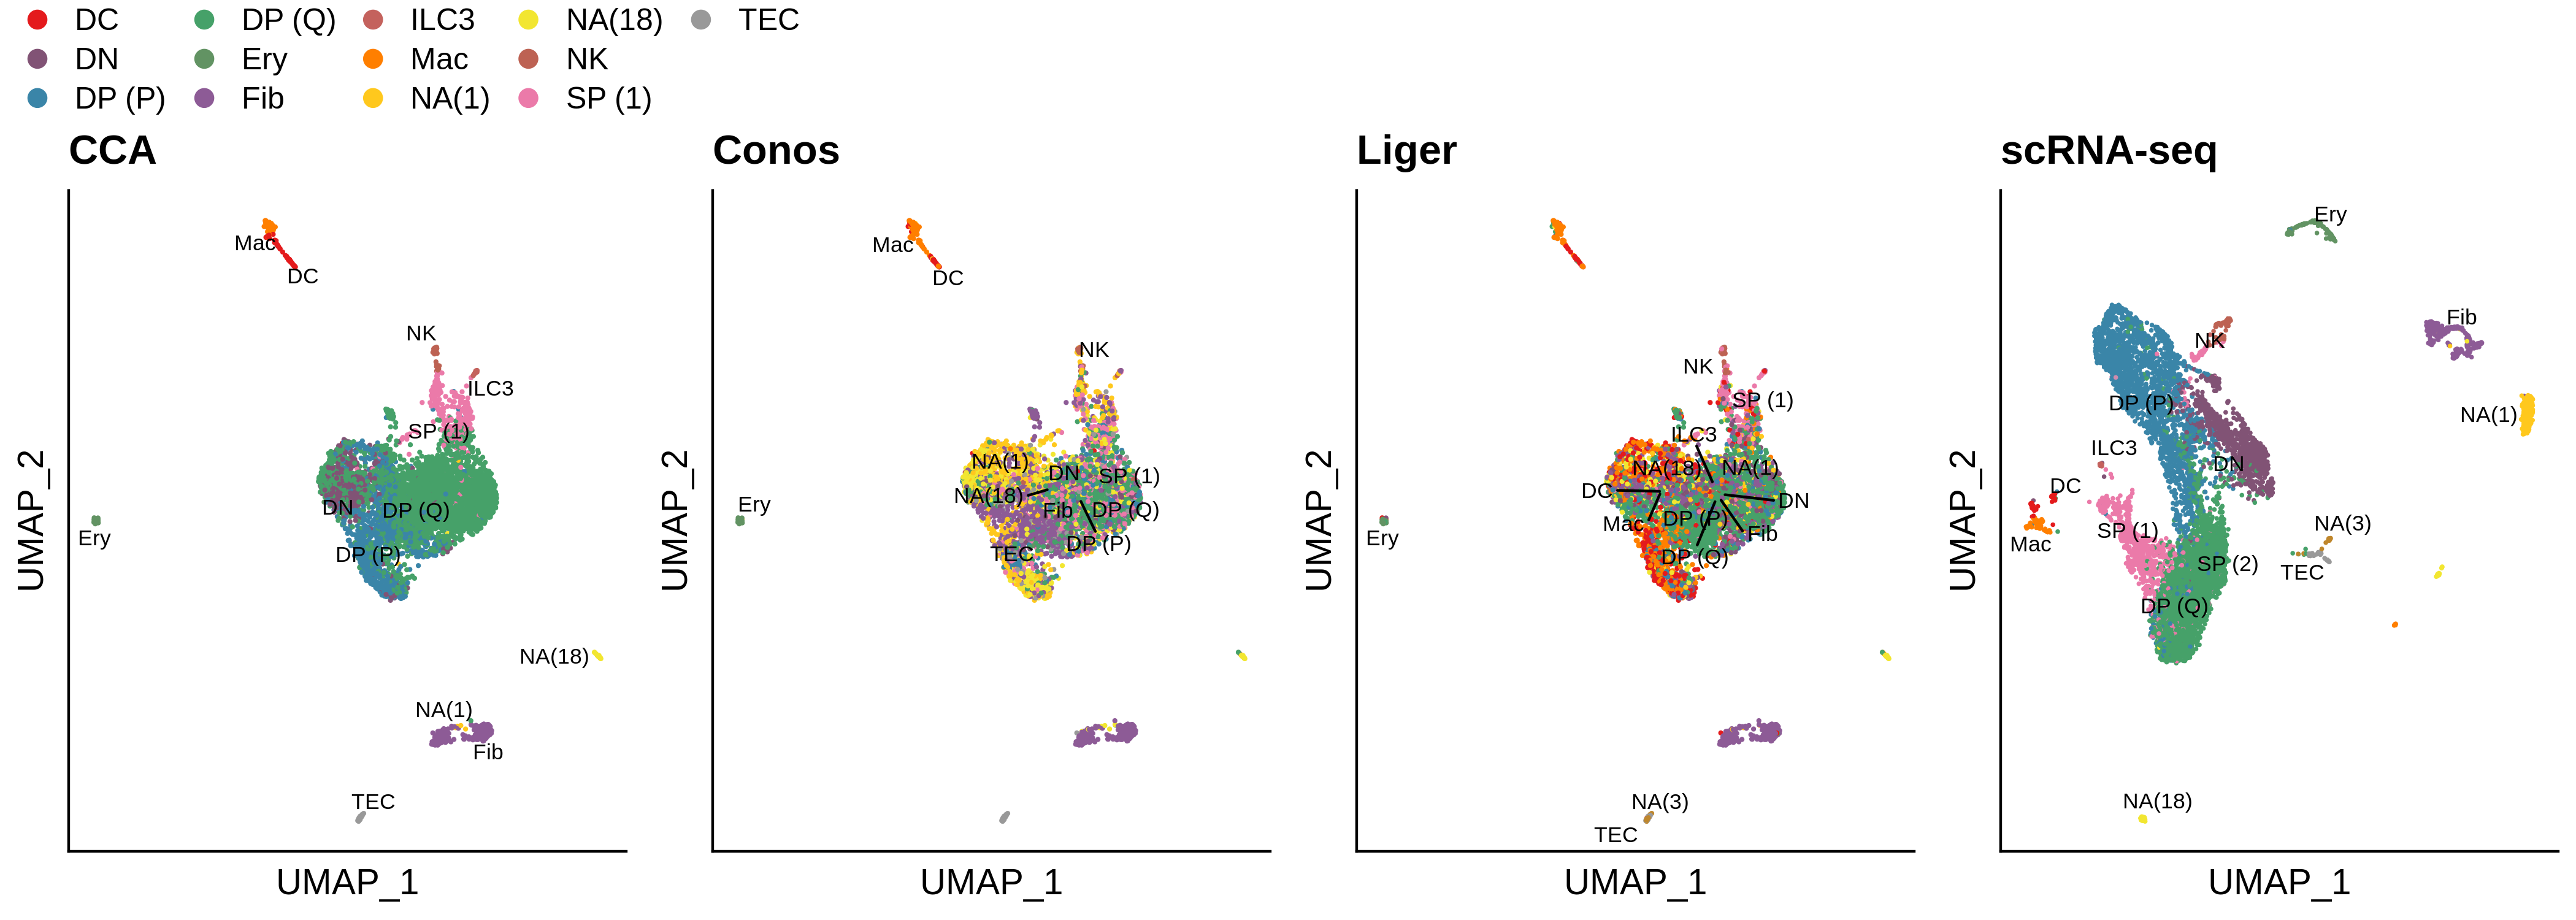
\includegraphics[width=66.67in]{../output/20191106_labelTransferEDA_PBMC/umap_labels} \caption{UMAP of ATAC}\label{fig:label-transfer-umap}
\end{figure}

All integration methods measure the uncertainty of their assignment
(Fig.@ref(fig:predict-score)A). Setting a threshold on the label
prediction score allows to remove from downstream analysis cells with a
low confidence prediction label, and mark them as unasssigned. We found
that at the cutoff of 0.5, suggested by Stuart et al.
(\protect\hyperlink{ref-stuartComprehensiveIntegrationSingleCell2019a}{2019}),
Liger excludes the least amount of cells, while Conos scores the most
cells with higher confidence (Fig.@ref(fig:predict-score)B).

\begin{figure}
\centering
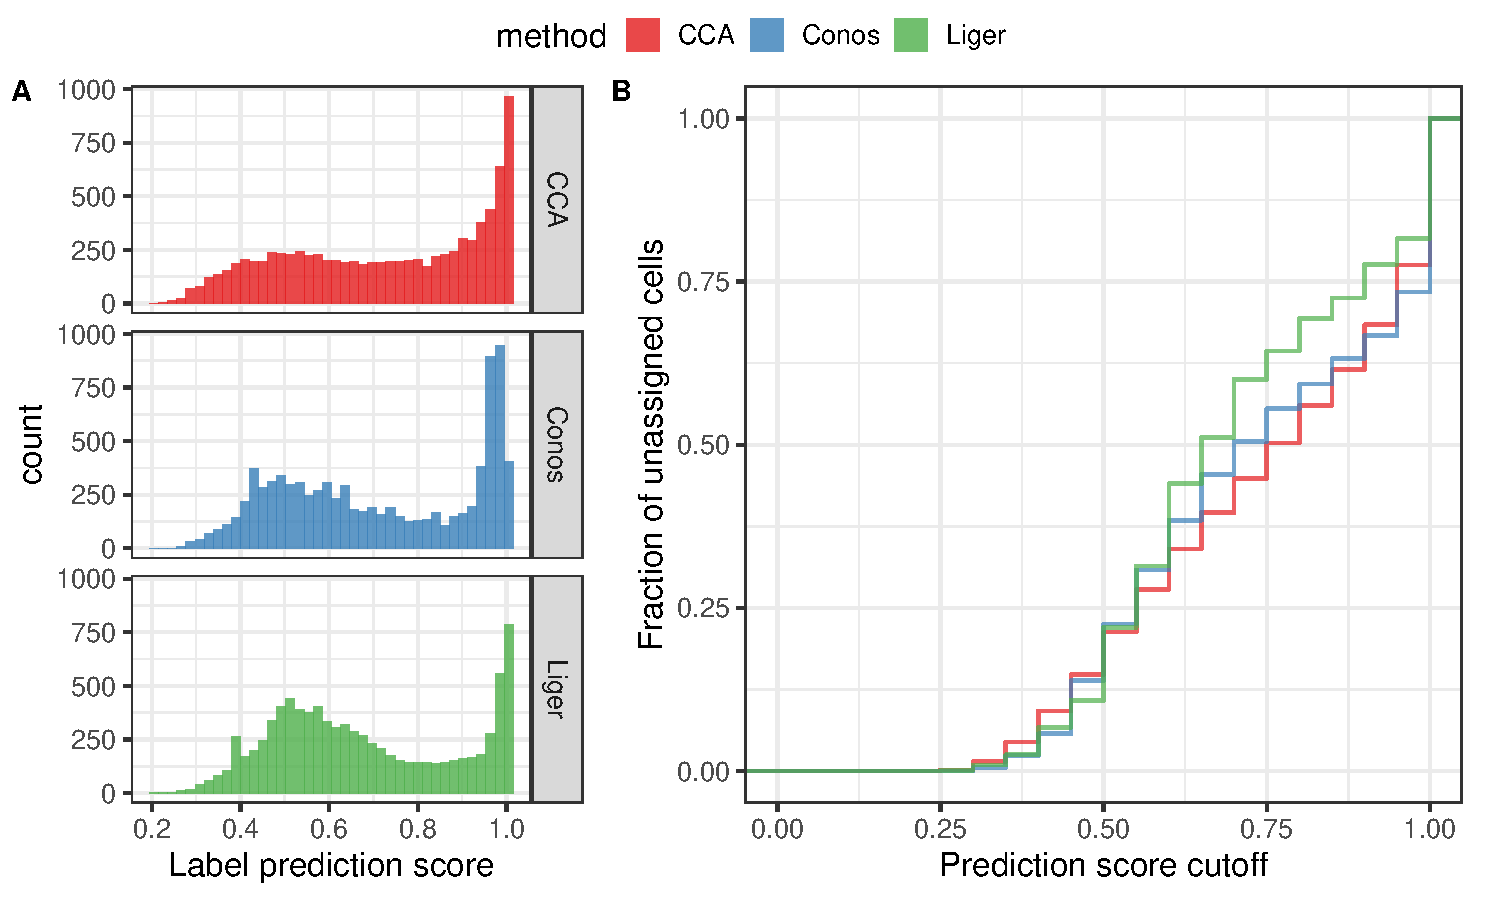
\includegraphics{../output/20191106_labelTransferEDA_PBMC/prediction_score_distribution.pdf}
\caption{Distribution of prediction scores for each method}
\end{figure}

\begin{figure}
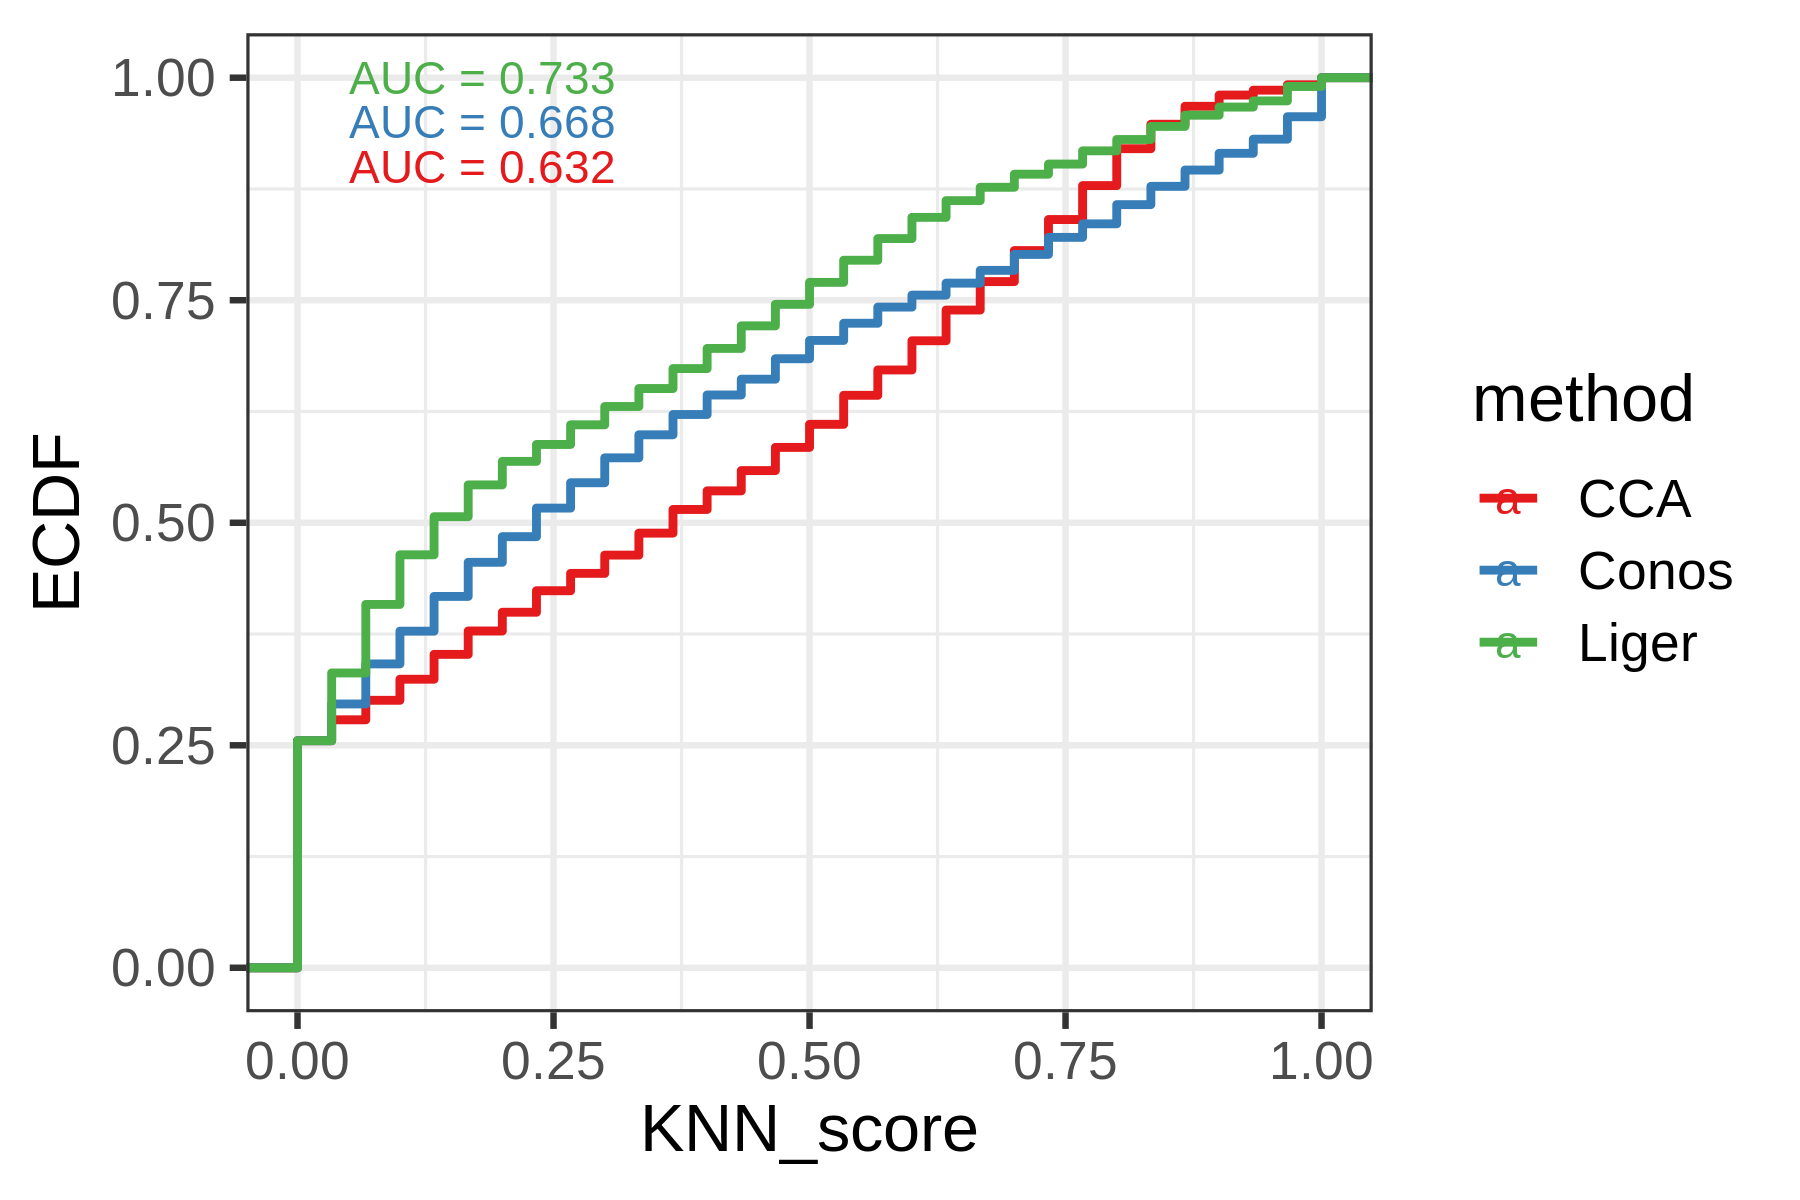
\includegraphics[width=25in]{../output/20191106_labelTransferEDA_PBMC/ KNN_score_ecdf_referenceHVG} \caption{Simulated data analysis}\label{fig:simdata}
\end{figure}

\hypertarget{methods}{%
\section{Methods}\label{methods}}

\hypertarget{dataset-details}{%
\subsection{Dataset details}\label{dataset-details}}

Incl. stats about dataset quality (median no. of fragments per cell,
perc. of fragments mapping to peaks, median no. of fragments in peaks
per cell)

\hypertarget{data-preprocessing}{%
\subsection{Data preprocessing}\label{data-preprocessing}}

\hypertarget{atac-seq}{%
\subsubsection{ATAC-seq}\label{atac-seq}}

ATAC-seq data is inherently sparse and noisy, more so than RNA-seq data.
In addition, methods for alignment with scRNA-seq data mostly require to
reduce accessibility signal to gene-level features. Different papers use
different strategies to preprocess ATAC-seq data and featurization
(benchmarked by Chen et al.
(\protect\hyperlink{ref-chenAssessmentComputationalMethods2019a}{2019})):

\begin{itemize}
\tightlist
\item
  \textbf{Seurat pipeline}: raw 10x sequencing reads were preprocessed
  to call peaks with Cellranger (v \ldots). Then all counts in peaks are
  summed up all counts in peaks within gene bodies + 2kb upstream (Welch
  et al.
  \protect\hyperlink{ref-welchSingleCellMultiomicIntegration2019a}{2019};
  Stuart et al.
  \protect\hyperlink{ref-stuartComprehensiveIntegrationSingleCell2019a}{2019}).
\item
  \textbf{SNAP-ATAC pipeline:} the genome is binned, then a cell x bin
  binary matrix is constructed. From this binary matrix a gene-level
  matrix is made (``Fast and Accurate Clustering of Single Cell
  Epigenomes Reveals Cis-Regulatory Elements in Rare Cell Types,''
  \protect\hyperlink{ref-FastAccurateClusteringa}{n.d.}).
\item
  \textbf{PCA based on bulk:} some studies (Buenrostro et al.
  \protect\hyperlink{ref-buenrostroIntegratedSingleCellAnalysis2018}{2018})
  find principal components of differentiation/cell type from bulk
  ATAC-seq datasets and then project the single-cells on the same space.
  Arguably, this will lead to miss out on accessibility dynamics of rare
  cell populations.
\item
  \textbf{LSI method:} this procedure starts by making a bin x cell
  matrix. Then normalization and rescaling are done using term
  frequency-inverse document frequency transformation (something from
  text mining), then SVD is performed to obtain a PC x cell matrix. This
  is used to cluster cells and peaks are called on the clusters. Then
  the peak x cell matrix is used to do PCA again (I am getting dizzy).
\end{itemize}

\hypertarget{rna-seq}{%
\subsubsection{RNA-seq}\label{rna-seq}}

Both datasets where preprocessed with std steps: removal of empty/lowQ
cells, normalization per cell coverage,

\hypertarget{feature-selection}{%
\paragraph{Feature selection}\label{feature-selection}}

\begin{itemize}
\tightlist
\item
  Highly-variable genes in RNA
\item
  genes that are expressed only in a few cells
\item
  Also ATAC specific markers are informative, contain signal from known
  marker genes in thymic development. Probably beneficial for alignment
  to take the union and not only the HVGs from RNA.
\end{itemize}

\hypertarget{tested-integration-methods}{%
\subsection{Tested integration
methods}\label{tested-integration-methods}}

\begin{longtable}[]{@{}llcc@{}}
\toprule
\begin{minipage}[b]{0.17\columnwidth}\raggedright
Method\strut
\end{minipage} & \begin{minipage}[b]{0.14\columnwidth}\raggedright
Reference\strut
\end{minipage} & \begin{minipage}[b]{0.30\columnwidth}\centering
Included in benchmark\strut
\end{minipage} & \begin{minipage}[b]{0.28\columnwidth}\centering
Reason for Excluding\strut
\end{minipage}\tabularnewline
\midrule
\endhead
\begin{minipage}[t]{0.17\columnwidth}\raggedright
Seurat CCA\strut
\end{minipage} & \begin{minipage}[t]{0.14\columnwidth}\raggedright
Stuart et al.
(\protect\hyperlink{ref-stuartComprehensiveIntegrationSingleCell2019a}{2019})\strut
\end{minipage} & \begin{minipage}[t]{0.30\columnwidth}\centering
Yes\strut
\end{minipage} & \begin{minipage}[t]{0.28\columnwidth}\centering
/\strut
\end{minipage}\tabularnewline
\begin{minipage}[t]{0.17\columnwidth}\raggedright
LIGER\strut
\end{minipage} & \begin{minipage}[t]{0.14\columnwidth}\raggedright
Welch et al.
(\protect\hyperlink{ref-welchSingleCellMultiomicIntegration2019a}{2019})\strut
\end{minipage} & \begin{minipage}[t]{0.30\columnwidth}\centering
Yes\strut
\end{minipage} & \begin{minipage}[t]{0.28\columnwidth}\centering
/\strut
\end{minipage}\tabularnewline
\begin{minipage}[t]{0.17\columnwidth}\raggedright
Conos\strut
\end{minipage} & \begin{minipage}[t]{0.14\columnwidth}\raggedright
({\textbf{???}})\strut
\end{minipage} & \begin{minipage}[t]{0.30\columnwidth}\centering
Yes\strut
\end{minipage} & \begin{minipage}[t]{0.28\columnwidth}\centering
/\strut
\end{minipage}\tabularnewline
\begin{minipage}[t]{0.17\columnwidth}\raggedright
scGen\strut
\end{minipage} & \begin{minipage}[t]{0.14\columnwidth}\raggedright
Lotfollahi, Wolf, and Theis
(\protect\hyperlink{ref-lotfollahiScGenPredictsSinglecell2019}{2019})\strut
\end{minipage} & \begin{minipage}[t]{0.30\columnwidth}\centering
No\strut
\end{minipage} & \begin{minipage}[t]{0.28\columnwidth}\centering
Requires cell type annotation in both datasets\strut
\end{minipage}\tabularnewline
\begin{minipage}[t]{0.17\columnwidth}\raggedright
totalVI\strut
\end{minipage} & \begin{minipage}[t]{0.14\columnwidth}\raggedright
Gayoso et al.
(\protect\hyperlink{ref-gayosoJointModelRNA2019}{2019})\strut
\end{minipage} & \begin{minipage}[t]{0.30\columnwidth}\centering
No\strut
\end{minipage} & \begin{minipage}[t]{0.28\columnwidth}\centering
Requires multi-omic data from the same single-cells\strut
\end{minipage}\tabularnewline
\begin{minipage}[t]{0.17\columnwidth}\raggedright
BBKNN\strut
\end{minipage} & \begin{minipage}[t]{0.14\columnwidth}\raggedright
Polański et al.
(\protect\hyperlink{ref-polanskiBBKNNFastBatch}{n.d.})\strut
\end{minipage} & \begin{minipage}[t]{0.30\columnwidth}\centering
No\strut
\end{minipage} & \begin{minipage}[t]{0.28\columnwidth}\centering
Bad alignment during testing\strut
\end{minipage}\tabularnewline
\begin{minipage}[t]{0.17\columnwidth}\raggedright
Cusanovich2018\strut
\end{minipage} & \begin{minipage}[t]{0.14\columnwidth}\raggedright
Cusanovich et al.
(\protect\hyperlink{ref-cusanovichSingleCellAtlasVivo2018a}{2018})\strut
\end{minipage} & \begin{minipage}[t]{0.30\columnwidth}\centering
No\strut
\end{minipage} & \begin{minipage}[t]{0.28\columnwidth}\centering
Code unavailable\strut
\end{minipage}\tabularnewline
\bottomrule
\end{longtable}

\hypertarget{transfer-label}{%
\subsubsection{Label transfer}\label{transfer-label}}

One of the key tasks for integration methods is to be able to transfer
cell type annotations learnt from a reference to a query dataset. This
is especially useful if the query is a scATAC-seq dataset, where calling
of cell types based on prior knownledge on marker genes is often not
possible. Different models are adapted to transfer discrete cell state
labels derived from gene expression to cells measured with scATAC-seq.

\hypertarget{seurat-cca}{%
\subparagraph{Seurat CCA}\label{seurat-cca}}

Identified anchor pairs are weighted based on the query cell local
neighboorhood (the k nearest anchors) and the anchor score. The obtained
reference cells x query cells weight matrix is then multiplied by the
matrix of annotation x reference cells, to generate a query cell x
annotation matrix. This returns a prediction score for each class for
every cell in the query dataset, ranging from 0 to 1 (Stuart et al.
\protect\hyperlink{ref-stuartComprehensiveIntegrationSingleCell2019a}{2019}).

\hypertarget{liger}{%
\subparagraph{LIGER}\label{liger}}

While the authors do not describe a method for transferring discrete
labels, I adapted their strategy for feature imputation. I build a
cross-dataset KNN graph in the aligned factor space, then I assign each
query cell to the most abundant label between the k nearest neighbors in
the reference dataset (k=30). The prediction score for label \(l\) is
computed as the fraction of nearest neighbors that have the predicted
label. \[
score = \frac{count(l)}{k}
\] \#\#\#\#\# Conos Label transfer is treated as a general problem of
information propagation between vertices of the common graph (detailed
in ({\textbf{???}})). The label score is the label probability updating
during the diffusion process.

\hypertarget{metrics-for-comparison-of-integration-models}{%
\subsection{Metrics for comparison of integration
models}\label{metrics-for-comparison-of-integration-models}}

Problems: finding optimal distance metric for gene accessibility and
expression (correlation doesn't work, too sparse). (Or more general: how
to relate features from different datasets) Nearest neighbors in PCA?
How to make a nearest neighbor graph between modalities - MNN cosine
normalizes each batch and then calculates distances

\begin{itemize}
\tightlist
\item
  PCA on integrated space and find genes with high eigen values
\item
  How to denoise the ATAC data??
\end{itemize}

\begin{enumerate}
\def\labelenumi{\arabic{enumi})}
\setcounter{enumi}{1}
\tightlist
\item
  Robustness to different fractions of cells in ATAC dataset
\item
  Leave-one-out approach for imputed data
\item
  \textbf{Fraction of unassigned cells} (but how to distinguish
  unassigned and badly assigned?): prediction score from label transfer
\item
  \textbf{Joint clustering: purity of cell type annotation inside a
  cluster, mixing within the same cluster between different
  technologies}
\item
  \textbf{Robustness to parameter picking (e.g.~no. of factors)}
\item
  Agreement metric defined by Welch et al.~2019: compare KNN graph of
  single datasets with KNN graph in integrated space, then calculate how
  many of each cell's NNs in the single dataset graph are also NNs in
  the integrated graph. Welch et al.~compare NN graphs built with
  different factor models to compare CCA and LIGER performance. I build
  for all methods KNN graphs from the PCA projection of imputed values.
\item
  \textbf{Expression not at random of markers after integration:} is the
  structure that is clear in the RNA maintained after embedding w the
  ATAC? From idea of JP collaborator

  \begin{itemize}
  \tightlist
  \item
    Find marker genes from RNA only
  \item
    Measure non-random expression in RNA only
  \end{itemize}
\item
  \textbf{pySCENIC on RNA only or integration w ATAC seq}
\end{enumerate}

\hypertarget{ideas-for-less-agnostic-integration}{%
\subsection{Ideas for less ``agnostic''
integration}\label{ideas-for-less-agnostic-integration}}

\begin{enumerate}
\def\labelenumi{\arabic{enumi})}
\tightlist
\item
  Select only a certain lineage of cells (e.g.~that you can align in
  pseudotime)
\item
  Annotation of cell types also in ATAC-seq data (e.g.~to use scGen)
\item
  Considering enhancer accessibility (matching them to genes??)
\end{enumerate}

\hypertarget{biological-interpretation-of-integration}{%
\subsection{Biological interpretation of
integration}\label{biological-interpretation-of-integration}}

In Cusanovich et al.~2018 they identify differentially accessible sites
\& cluster specific accessibility patterns.

\hypertarget{other-random-things}{%
\subsection{Other random things}\label{other-random-things}}

\begin{itemize}
\tightlist
\item
  How does ATAC improve the RNA? Can we detect cell clusters/populations
  that are highly homogeneous in the RNA but display significant
  variability at the accessibility level? But what is variability in
  super noisy ATAC seq?
\item
  Studying pioneering TFs: temporal relationship between TF expression
  and accessibility (are they really opening chromatin?) Could be done
  on the time series data Svensson and Pachter
  (\protect\hyperlink{ref-svenssonInterpretableFactorModels2019}{2019})
\item
  Clonality of epigenetic modifications ATAC + TCR tracing
\end{itemize}

\hypertarget{bibliography}{%
\subsection*{Bibliography}\label{bibliography}}
\addcontentsline{toc}{subsection}{Bibliography}

\hypertarget{refs}{}
\leavevmode\hypertarget{ref-buenrostroIntegratedSingleCellAnalysis2018}{}%
Buenrostro, Jason D., M. Ryan Corces, Caleb A. Lareau, Beijing Wu,
Alicia N. Schep, Martin J. Aryee, Ravindra Majeti, Howard Y. Chang, and
William J. Greenleaf. 2018. ``Integrated Single-Cell Analysis Maps the
Continuous Regulatory Landscape of Human Hematopoietic
Differentiation.'' \emph{Cell} 173 (6): 1535--1548.e16.
\url{https://doi.org/10.1016/j.cell.2018.03.074}.

\leavevmode\hypertarget{ref-chenAssessmentComputationalMethods2019a}{}%
Chen, Huidong, Caleb Lareau, Tommaso Andreani, Michael E. Vinyard, Sara
P. Garcia, Kendell Clement, Miguel A. Andrade-Navarro, Jason D.
Buenrostro, and Luca Pinello. 2019. ``Assessment of Computational
Methods for the Analysis of Single-Cell ATAC-Seq Data.'' \emph{bioRxiv},
August, 739011. \url{https://doi.org/10.1101/739011}.

\leavevmode\hypertarget{ref-cusanovichSingleCellAtlasVivo2018a}{}%
Cusanovich, Darren A., Andrew J. Hill, Delasa Aghamirzaie, Riza M. Daza,
Hannah A. Pliner, Joel B. Berletch, Galina N. Filippova, et al. 2018.
``A Single-Cell Atlas of in~Vivo Mammalian Chromatin Accessibility.''
\emph{Cell} 174 (5): 1309--1324.e18.
\url{https://doi.org/10.1016/j.cell.2018.06.052}.

\leavevmode\hypertarget{ref-FastAccurateClusteringa}{}%
``Fast and Accurate Clustering of Single Cell Epigenomes Reveals
Cis-Regulatory Elements in Rare Cell Types.'' n.d., 41.

\leavevmode\hypertarget{ref-gayosoJointModelRNA2019}{}%
Gayoso, Adam, Romain Lopez, Zoë Steier, Jeffrey Regier, Aaron Streets,
and Nir Yosef. 2019. ``A Joint Model of RNA Expression and Surface
Protein Abundance in Single Cells.'' \emph{bioRxiv}, October, 791947.
\url{https://doi.org/10.1101/791947}.

\leavevmode\hypertarget{ref-lotfollahiScGenPredictsSinglecell2019}{}%
Lotfollahi, Mohammad, F. Alexander Wolf, and Fabian J. Theis. 2019.
``scGen Predicts Single-Cell Perturbation Responses.'' \emph{Nature
Methods} 16 (8): 715. \url{https://doi.org/10.1038/s41592-019-0494-8}.

\leavevmode\hypertarget{ref-polanskiBBKNNFastBatch}{}%
Polański, Krzysztof, Matthew D. Young, Zhichao Miao, Kerstin B. Meyer,
Sarah A. Teichmann, and Jong-Eun Park. n.d. ``BBKNN: Fast Batch
Alignment of Single Cell Transcriptomes.'' \emph{Bioinformatics}.
Accessed October 3, 2019.
\url{https://doi.org/10.1093/bioinformatics/btz625}.

\leavevmode\hypertarget{ref-stuartComprehensiveIntegrationSingleCell2019a}{}%
Stuart, Tim, Andrew Butler, Paul Hoffman, Christoph Hafemeister,
Efthymia Papalexi, William M. Mauck, Yuhan Hao, Marlon Stoeckius, Peter
Smibert, and Rahul Satija. 2019. ``Comprehensive Integration of
Single-Cell Data.'' \emph{Cell} 177 (7): 1888--1902.e21.
\url{https://doi.org/10.1016/j.cell.2019.05.031}.

\leavevmode\hypertarget{ref-svenssonInterpretableFactorModels2019}{}%
Svensson, Valentine, and Lior Pachter. 2019. ``Interpretable Factor
Models of Single-Cell RNA-Seq via Variational Autoencoders.'' Preprint.
Bioinformatics. \url{https://doi.org/10.1101/737601}.

\leavevmode\hypertarget{ref-welchSingleCellMultiomicIntegration2019a}{}%
Welch, Joshua D., Velina Kozareva, Ashley Ferreira, Charles Vanderburg,
Carly Martin, and Evan Z. Macosko. 2019. ``Single-Cell Multi-Omic
Integration Compares and Contrasts Features of Brain Cell Identity.''
\emph{Cell} 177 (7): 1873--1887.e17.
\url{https://doi.org/10.1016/j.cell.2019.05.006}.


\end{document}
